\chapter{Úvod}

Nanotechnologie je jeden z nejčastěji skloňovaných pojmů v dnešním technickém světě. Internetový vyhledávač Google.com nabízí po zadání slova "nanotechnologie"$\,$ 5,9 milionu výsledků vyhledávání. Anglická verze "nanotechnology"$\,$ nabízí dokonce 43,8 milionu výsledků vyhledávání. Za otce nanotechnologií je považován americký fyzik Richard P. Feynman, který v roce 1959 představil myšlenku nanotechnologií Americké fyzikální společnosti na přednášce s názvem {\it There’s Plenty of Room at the Bottom}. \cite{britanica_nanotechnology} 
Pojem nanotechnologie poprvé použil až v roce 1974 profesor univerzity v Tokyu Norio Taniquchi. \cite{timeline_nanotechnology}\\

Nanotechnologie jsou interdisciplinární obor, který nachází své uplatnění v různých oblastech lidské činnosti. Hovoříme o nanotechnologiích v biologii a medicíně, elektronice, informatice a komunikacích, energetice, materiálových vědách, v průmyslu, v oblasti znečištění i ochrany životního prostředí. \cite{whats_nanotechnology} \\

Podstatou nanotechnologií je jejich malý rozměr. Obecně uznávanou definicí je, že rozměr nanotechnologií musí být ve všech třech dimenzích, nebo alespoň ve dvou dimenzích, menší než 100$\,$nm. Na obrázcích \ref{fig:scale_osa_1} a \ref{fig:scale_osa_2} na další straně je vidět srovnání velikostí konkrétních příkladů, pro lepší představivost o jak malé rozměry se jedná. \\

Velký rozvoj nanotechnologií umožnil rozvoj zobrazovacích metod, které jsou nyní schopné zobrazovat v nanometrovém rozlišení a také jsme schopni pohybovat a ovlivňovat jednotlivé atomy. V roce 1981 Gerd Binnig a Heinrich Rohrer představili skenovací tunelovací mikroskop. 80. léta tak odstartovala vývoj nanotechnologií \cite{timeline_nanotechnology}. Rozvoj nanotechnologií je také spojen s rozvojem nových analytických metod, které jsou schopné charakterizovat nové materiály.\\

V této práci se budu zabývat obecným využitím nanotechnologií, systémem hodnocení rizik, důležitými faktory ovlivňující toxicitu a ekotoxicitu nanomateriálů.

    \begin{figure}
        \centering
        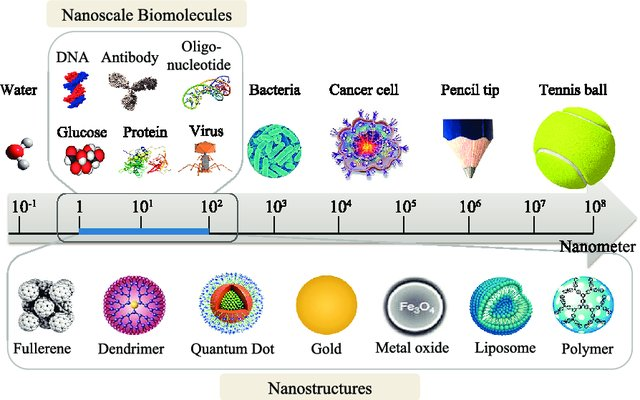
\includegraphics[width=0.87\textwidth]{pictures/Nanoscale-integration-of-nanoparticles-and-biomolecules_W640.jpg}
        \caption{Schéma rozměrové osy. \cite{saallah2018}}
        \label{fig:scale_osa_1}
    \end{figure}
    
    \begin{figure}
        \centering
        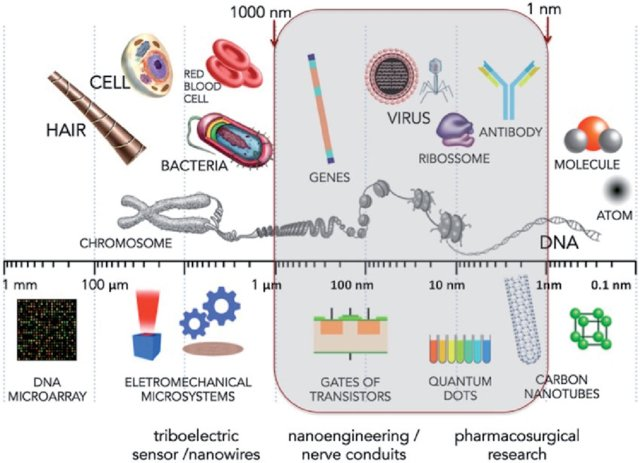
\includegraphics[width=0.87\textwidth]{pictures/Scheme-with-nanoscale-comparison-Nanotechnology-are-related-to-the-study-extremely-small_W640.jpg}
        \caption{Schéma rozměrové osy. \cite{mendonca2017}}
        \label{fig:scale_osa_2}
    \end{figure}